\documentclass{article}
\usepackage{graphicx} % Required for inserting images
\usepackage{verbatim}
\usepackage{fancyvrb}
\usepackage{listings}
\usepackage{tabularx}


\usepackage{xcolor}
\definecolor{codegreen}{rgb}{0,0.6,0}
\definecolor{codegray}{rgb}{0.5,0.5,0.5}
\definecolor{codeorange}{rgb}{1,0.49,0}
\definecolor{backcolour}{rgb}{0.95,0.95,0.96}

\usepackage{etoolbox} %for big tit-le

\makeatletter
\patchcmd{\@maketitle}{\LARGE}{\Huge}{\typeout{OK 1}}{\typeout{Failed 1}}
\patchcmd{\@maketitle}{\large \lineskip}{\Large \lineskip}{\typeout{OK 2}}{\typeout{Failed 2}}
\makeatother

\lstdefinestyle{mystyle2}{
    backgroundcolor=\color{backcolour},   
    commentstyle=\color{cyan},
    keywordstyle=\color{blue},
    numberstyle=\tiny\color{codegray},
    stringstyle=\color{magenta},
    basicstyle=\ttfamily\footnotesize,
    breakatwhitespace=false,         
    breaklines=true,                 
    captionpos=b,                    
    keepspaces=true,                 
    numbers=left,                    
    numbersep=5pt,                  
    showspaces=false,                
    showstringspaces=false,
    showtabs=false,                  
    tabsize=2,
    xleftmargin=10pt,    
}

\lstdefinestyle{mystyle3}{
    backgroundcolor=\color{backcolour},   
    commentstyle=\color{cyan},
    keywordstyle=\color{purple},
    numberstyle=\tiny\color{codegray},
    stringstyle=\color{blue},
    basicstyle=\ttfamily\footnotesize,
    breakatwhitespace=false,         
    breaklines=true,                 
    captionpos=b,                    
    keepspaces=true,                 
    numbers=left,                    
    numbersep=5pt,                  
    showspaces=false,                
    showstringspaces=false,
    showtabs=false,                  
    tabsize=2,
    xleftmargin=10pt,    
}

\title{CSN-291\\Assignment I}
\author{Garv Sethi\\22115057\and Mmukul
Khedekar\\22114054\and Granth Gaud\\22114035\and Atharv Joshi\\22114012 \and Divyansh Verma\\22114033 }
\date{}
\begin{document}

\maketitle
\clearpage
\begin{center}
\section*{Stubs and drivers generator for object oriented program testing using sequence and class diagrams}
\end{center}
\subsection*{Authors and Credits: }
Peerawut Luengruengroj and Taratip Suwannasart from the department of computer engineering,
faculty of engineering,
Chulalongkorn University. The paper under discussion was originally published in 2018 5th International Conference on Computational Science/ Intelligence and Applied Informatics (CSII).

\section{Prelude to the paper}
%humpe(mention testing waala part here)
The typical stages in any software development life cycle are \cite{r2} :\\

\begin{enumerate}
    \item \textbf{Requirements Analysis:}These include understanding the project's goals, user's needs and defining the system's requirements.
    \item \textbf{System Design:} Creating a high-level design of the system architecture and making design decisions.
    \item \textbf{Implementation (Coding):} Writing code based on design specifications and best practices.
    \item \textbf{Testing:} Verifying the software for correctness and identifying defects.
    \item \textbf{Deployment:} Preparing the software for release and deploying it to the production environment.
    \item \textbf{Maintenance and Support:} Addressing issues, implementing updates and providing an ongoing support.
\end{enumerate}


% 1. \\

% 2. \\

% 3. \\

% 4. \\

% 5. \\

% 6. \\

Among all these stages, testing is a critical phase in the software development process that aims to verify the correctness, functionality, and reliability of a software system. It involves systematically evaluating the software to identify defects, ensure it meets the requirements and provide confidence that it works as intended. Testing is performed throughout the development life cycle and helps improve the software quality. \\

\textbf{Types of Testing: }\\
% • Unit Testing\\
% • Integration Testing\\
% • System Testing\\
% • Acceptance Testing\\
% • Regression Testing\\
% • Performance Testing\\
% • Security Testing\\
% • Usability Testing\\
% • Exploratory Testing\\

\begin{tabularx}{\textwidth}{
    @{\hspace{1.5em}}
    >{\leavevmode\llap{\textbullet~}\raggedright}
    X
    @{\quad\hspace{1.5em}}
    >{\leavevmode\llap{\textbullet~}\raggedright\arraybackslash}
    X
    @{}
  }
  Unit Testing & Integration Testing \\
  System Testing & Acceptance Testing \\ 
  Regression Testing & Performance Testing \\ 

  Security Testing & Usability Testing \\
  Exploratory Testing \\
\end{tabularx}

Among these types of testing, \textbf{Unit Testing} is a fundamental testing approach in software development where individual units or components of a software system are tested in isolation to ensure that they work as expected. A unit typically refers to a function, method, or module within the code. The primary goal of unit testing is to validate that each unit of the software performs its intended functionality correctly. There are two ways in which unit testing could be conducted and they are compared on the basis of their efficiency below.\\

\textbf{Manual versus Automated Unit Testing: }\\

• Manually creating and executing unit tests can be tedious, especially as the codebase grows. It's time-consuming, error-prone, and becomes impractical when dealing with complex systems.\\

• Automated unit testing is preferred because it's efficient and repeatable. Automated tests ensure that the units continue to work as expected as our code continues to evolve.\\


\section{Executive Summary}
%toh(explained in the title)
In an object-oriented software development, unit test cases involve calling the method of each class and examining whether the produced results are consistent with the expected results. However, the software under testing may contain a ton of classes with each method being invoked within a class or between different classes. It could require a lot of time to create a stub and a driver for testing each object.\\

There are related tools that can create stubs and drivers from UML diagrams but these tools either require source code information or can identify stubs and drivers from UML diagrams but cannot generate them automatically.\\

The primary objective of the paper is to introduce a tool for generating stubs and drivers that use  UML (Unified Modeling Language) sequence diagrams and class diagrams to streamline the process, enabling testers to create stubs and drivers more efficiently based upon the relationships among classes and method calls.\\


\begin{itemize}
    \item \textbf{Stub:} A stub is a piece of throwaway code that emulates or imitates a called unit. Stubs simulate the behavior of dependent components that are not yet developed or available for testing. It basically imitates a unit which is called by a unit test case.
    \item \textbf{Driver:} A driver is a module that contains wired-in test inputs, calls the module being tested and displays the outputs or compares the actual output with the expected output. It basically imitates a unit which calls the unit under testing.
    \item \textbf{Call Graph:} A call graph is a directed-control flow graph which depicts the relationship between the subroutine inside the program. Each node refers to a function or method and each directed-edge refers to a function calling. 
\end{itemize}
    
% \\

% \\


\begin{figure}
    \centering
    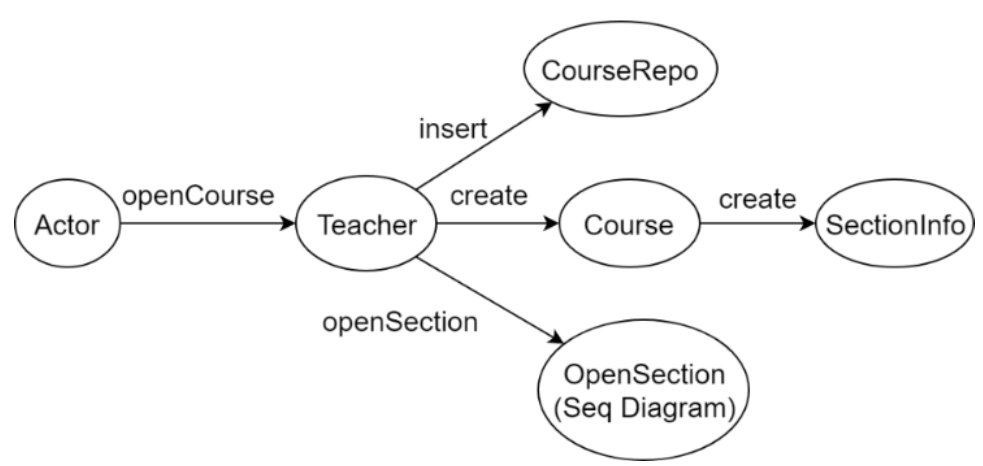
\includegraphics[scale=0.43]{Untitled.png}
    \caption{A Typical Call Graph}
    \label{fig:enter-label}
\end{figure}


Various related research works were published in this domain.
These research papers introduce different approaches to improve software testing and test suite coverage. They explore the creation of stubs, drivers, and test cases, as well as techniques for generating test suites using UML diagrams and symbolic execution. However, there are some limitations, such as the need for a complete source code or the manual creation of the original test suite in some cases.\\
\\ 

\textbf{STUBS AND DRIVERS GENERATION TOOL : }\\

The paper describes a tool called \textbf{Stubs and Drivers Generation Tool} which can be used to automate unit testing. It is a web application. The procedure is as follows :\\

\begin{enumerate}
    \item The tool imports UML sequence and class diagrams in XML files.
    \item The tool will process the sequence diagrams in the XML file to identify the objects, messages and method calls involved in the sequence diagram to create a call graph.
    \item The tool will process the class diagrams in the XML file to identify the packages, classes and method signatures.
    \item The tool will use objects and messages data from the sequence diagram to create the call graph and save it into the database.
    \item Testers can choose a class to test and specify if they want the tool to generate stubs or drivers. The tool processes the call graph to identify which classes need stubs or drivers. For a class under test, if the tester chooses to create stub, a stub for the called class will be created and if the tester chooses to create a driver, a driver will be created for a class which calls the class under test.
    \item The tool will create source code depending on source code type (Stub or Driver) and a source code language. The generated source code can be customized by testers.
    
    
\end{enumerate}

% 1. \\

% 2. \\

% 3. \\

% 4. \\

% 5.  \\

% 6. \\



\section{Implementation}
%hai(explained in the title)
The tool discussed in the paper was deployed using JavaScript and PHP and is run as a web-based application. The tool uses a MySQL database to store the uploaded XML files, processed diagram data (sequence and class diagrams), call graphs and generated source code. This allows for data persistence and future editing.\\


The tool aims to aid the software engineer by auto generating stubs and driver classes \cite{diggaD} and thus ease the testing process. The tool processes the XML file which is provided to it and uses it to generate a \textit{'Call Graph'} which is essentially a hierarchy structure involving different objects and how different function calls are made between them. This graph is also stored in the MySQL database along with the other XML files and class diagrams and the generated source codes.\\

Upon uploading the XML diagrams to the database, the tester can choose the sequence diagram and class diagram that contain the class under test. The user chooses a target class, defines the filename for a generated stub or driver, specifies the source code nature (Stub or Driver) and selects the desired object oriented programming language (for example, Java or C++).\\

After the source code is generated the tester can edit the generated source code by setting default/random values and return types, more explanation on this is provided in sections 3.1 and 3.2 . Source code is by default saved to the database for future revisions.\\


Before moving onto the actual generator functioning it would be best to see how a simple stub/ driver is implemented in C++.
\lstinputlisting[language=C++,mathescape=true, firstline=1,style=mystyle2]{stublol.cpp}
Here we have a stub class which for the purposes of testing always returns true and hence we can test our encryption class, although we must always remember that stub is a temporary class and we must also actually implement the functionality of the class.
\subsection{Stub Generation}
The tool generates individual stubs by comparing a message in a call graph to a message in the class diagram. Firstly we flush the input values to the console and then we return a randomized value depending upon the return type. If the return type is void we omit from returning anything and if it returns an object then we return a NULL pointer \cite{newnig}.
\lstinputlisting[language=C++,mathescape=true, firstline=1,style=mystyle3]{newlol.cpp}
\subsection{Driver Generation}
The tool creates each driver by matching an invoked message with a method in the class diagram and subsequently generates a code to execute the respective method. In the case where the method includes a parameter, the tool will generate a random value corresponding to the data type of the parameter. If the parameter itself is an object, the tool will utilize NULL pointer as the input value.
\lstinputlisting[language=C++,mathescape=true, firstline=1,style=mystyle3]{newlollol.cpp}


\section{Perks of this methodology}
%hi(positive points)
Stubs and Drivers are an integral part of unit testing. Unit testing, as explained above, is done to test each individual units (or components) of the software system. Moreover, it is performed at the time of development to reduce the testing time and cost after the software has been developed. In fact, unit testing is performed by the developers themselves.\\

Since, it is performed at the time of testing, it may be possible that each component of the software has been already implemented successfully. It may also be possible that a module or a class shares some common functionality with an incomplete module or a class. In such cases it becomes difficult to isolate the module and test its functionality. This is where stubs and drivers are essentially used. We need them to isolate a module under testing and check its functionality.\\

Another difficulty that's encountered even after having the stubs and drivers implemented is that a software program can have hundreds of thousands of classes. Hence, it may not be possible to manually generate stubs and drivers for such a large number of classes. It should also be noted that we might not have the entire code for our program with us while we are conducting the testing upon it. But we can have the sequence diagrams and class diagrams created before we start implementing the software program.\\

The Stubs and Drivers Generation Tool takes the aforementioned challenges into consideration to ensure a smooth testing procedure. This is the inherent advantage of this tool that results in the following outcomes:-

\begin{enumerate}
    \item The programmers can refine the code and can cross-verify that the modules work properly. 
    \item \textbf{Early Detection of Issues:} Developers can identify issues at an early stage, preventing them from escalating into more complex and challenging problems to resolve.
    \item This provides the developers with confidence in their code as they can validate that each unit is working as expected.
    \item \textbf{Faster Development:} Developers don’t have to wait for the entire software program to be developed. They can make desired changes in a module at the time of implementation.
    \item \textbf{Facilitation of Refactoring:} Developers can make changes safely to the code, as they can validate that their changes don’t break existing functionality.
    \item \textbf{Parallel Development:} Different teams can work on different components simultaneously.
    \item \textbf{Faster Testing:} Since stubs and drivers have a simplified implementation of the original module, this improves the speed of testing.
    \item \textbf{Testing Error Handling:} Stubs can be configured to return specific error conditions allowing developers to test error-handling mechanisms in their code.
\end{enumerate}




\section{Gaps in this methodology}

A  tool designed for the purpose of creating stubs and drivers, which are essential components in software development, can potentially exhibit certain limitations and disadvantages that need to be considered. Stubs and drivers are integral to the process of testing and integrating different parts of software applications. However, despite their importance, using a tool exclusively for developing stubs and drivers can come with several drawbacks:

\begin{enumerate}

\item \textbf{Incomplete Behavior:} Stubs and drivers are simplified versions of components that may not completely replicate the behavior of the actual components. This can lead to incomplete testing, as certain functionalities or interactions may not be accurately represented, potentially resulting in undiscovered bugs.

\item \textbf{Inflexibility:} The tool might offer limited flexibility when it comes to generating stubs and drivers. Developers may require custom behaviors or specific variations that the tool cannot accommodate, leading to workarounds or manual adjustments.

\item \textbf{False Positives and Negatives:} Due to their simplified nature, stubs and drivers can sometimes produce false positives (indicating that a component works correctly when it doesn't) or false negatives (indicating a problem when there isn't one) in the testing process. This can lead to confusion and wasted effort in debugging.

\item \textbf{Limited Testing Scope:} Stubs and drivers are generally designed to facilitate testing of individual components in isolation. However, many software defects can emerge when different components interact. Stubs and drivers may not adequately simulate these interactions, leading to potential issues being missed.

\item \textbf{Scalability Concerns:} The tool's performance and effectiveness might degrade as the project scales up in complexity and size. This can lead to bottlenecks in the development process and hinder project progress.

\item \textbf{Maintenance Efforts:} The tool itself requires maintenance, updates, and support. If it's not actively maintained, it might lead to compatibility issues with newer development platforms and languages.

\item \textbf{Dependency Risk:} Over-reliance on a single tool can become a risk if the tool becomes obsolete, unsupported, or its development is halted. This can lead to a scramble to find alternatives or adapt to new tools.

\item \textbf{Costs:} Depending on the tool's licensing model, it might come with financial costs. These costs could become a burden on project budgets, especially for smaller teams or organizations with limited resources.

\end{enumerate}



\section{Concluding Remarks}
%:P (lol)
%mmukul nigg get to work!
%me at 5am

We have conclusively presented a procedure to generate stubs and drivers to test the target units of the desired program solely based on the information of the sequence and class diagrams of our program that are stored in the XML files that we would provide to the tool. We have discussed the importance and necessity of unit testing as well as the pivotal role that stubs and drivers play in the process of testing. \\ 

The tool's architecture and functioning are explained along with an illustrative code to aid the demonstration. Furthermore, the benefits of the tool have also been highlighted. We particularly think that this tool could improve and speed-up the testing process in software development and could have a significant impact upon the software industry as it could create a room for parallel development and reliable verification of the functionality of the units. \\

While there are many benefits of this tool, we have also presented the limitations of this tool in terms of its effectiveness and its region of applicability. The tool is designed to operate optimally under ideal conditions and does not particularly consider various unforeseen real-world scenarios where it would be eventually applied. \\

The acknowledgment of both the positive and negative aspects of the tool allows scope for further enhancements in the future. Its ability to automatically generate accurately working stubs and drivers could be a key-goal during the future improvements thereby, minimising the manual interference in situations when false-positive and negative stubs and drivers are generated. Another aspect that could be worked upon is to generate accurate stubs and drivers with even less detailed sequence and class diagrams. \\

In conclusion, the tool aims to simplify unit testing in object-oriented software development and offers the potential for improved testing efficiency, early issue detection and enhanced software quality. However, it's important to recognize the tool's limitations and consider its application within the broader context of software testing and development. 

\section*{Individual Contribution}
\begin{enumerate}
    \item \textbf{Mmukul Khedekar:} Prelude to the paper 
    \item \textbf{Divyansh Verma: } Executive Summary 
    \item \textbf{Garv Sethi:}  Implementation
    \item \textbf{Atharv Joshi: } Perks of this methodology
    \item \textbf{Granth Gaud: } Gaps in this methodology
     
\end{enumerate}
\bibliographystyle{plain}
\bibliography{ref}


\end{document}
